\section{SurveySessionAbstract Klassenreferenz}
\label{classSurveySessionAbstract}\index{SurveySessionAbstract@{SurveySessionAbstract}}
Klassendiagramm für SurveySessionAbstract::\begin{figure}[H]
\begin{center}
\leavevmode
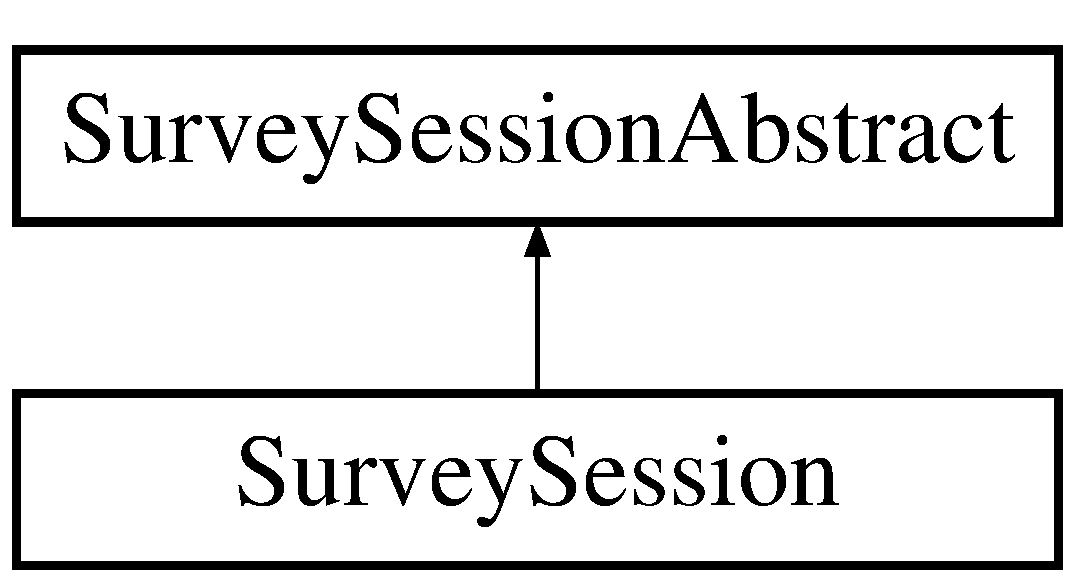
\includegraphics[height=2cm]{classSurveySessionAbstract}
\end{center}
\end{figure}
\subsection*{Öffentliche Methoden}
\begin{CompactItemize}
\item 
{\bf SurveySessionAbstract} (\$id=null)
\item 
{\bf getId} ()
\item 
{\bf getSurvivorEmail} ()
\item 
{\bf getTid} ()
\item 
{\bf getFinished} ()
\item 
{\bf getValue} (\$key)
\item 
{\bf getSurveyId} ()
\item 
{\bf getSurveyLanguage} ()
\item 
{\bf getSurveyData} ()
\item 
{\bf setDataSource} (\$sourceName=null)
\item 
{\bf setValue} (\$key, \$value)
\item 
{\bf \_\-loadDataById} (\$id)
\item 
{\bf \_\-loadDataByTid} (\$tid)
\item 
{\bf \_\-validateInput} (\$key, \$value)
\item 
{\bf \_\-delete} (\$id)
\item 
{\bf \_\-insertSurveyData} (\$key)
\item 
{\bf \_\-updateSurveyData} (\$id, \$key, \$value)
\item 
{\bf getLastError} ()
\end{CompactItemize}
\subsection*{Öffentliche Attribute}
\begin{CompactItemize}
\item 
{\bf \$\_\-lastError}
\item 
{\bf \$\_\-TABLE\_\-SDATA}
\item 
{\bf \$survivorId}
\item 
{\bf \$surveyId}
\item 
{\bf \$emailSent}
\item 
{\bf \$survivorEmail}
\item 
{\bf \$tid}
\item 
{\bf \$finished}
\end{CompactItemize}


\subsection{Ausführliche Beschreibung}
de.mksurvey - classes \begin{Desc}
\item[Version:]\$Id:\$\end{Desc}
Copyright (c) 2007 M.Kupriyanov \begin{Desc}
\item[Autor:]Mikhaylo Matiyenko-Kupriyanov, $<${\tt m@kupriyanov.de}$>$ \end{Desc}
\begin{Desc}
\item[Datum:]15.07.2007 18:15:58 \end{Desc}


Definiert in Zeile 16 der Datei class.SurveySesionAbstract.php.

\subsection{Dokumentation der Elementfunktionen}
\index{SurveySessionAbstract@{SurveySessionAbstract}!SurveySessionAbstract@{SurveySessionAbstract}}
\index{SurveySessionAbstract@{SurveySessionAbstract}!SurveySessionAbstract@{SurveySessionAbstract}}
\subsubsection{\setlength{\rightskip}{0pt plus 5cm}SurveySessionAbstract.SurveySessionAbstract (\$ {\em id} = {\tt null})}\label{classSurveySessionAbstract_7c5482c5e26ebdc8dc53eb0fbd28b70c}




Definiert in Zeile 31 der Datei class.SurveySesionAbstract.php.

Benutzt \_\-loadDataById().\index{SurveySessionAbstract@{SurveySessionAbstract}!getId@{getId}}
\index{getId@{getId}!SurveySessionAbstract@{SurveySessionAbstract}}
\subsubsection{\setlength{\rightskip}{0pt plus 5cm}SurveySessionAbstract.getId ()}\label{classSurveySessionAbstract_a7d9a6ad83cb2a401a7cd81bc724df60}




Definiert in Zeile 44 der Datei class.SurveySesionAbstract.php.\index{SurveySessionAbstract@{SurveySessionAbstract}!getSurvivorEmail@{getSurvivorEmail}}
\index{getSurvivorEmail@{getSurvivorEmail}!SurveySessionAbstract@{SurveySessionAbstract}}
\subsubsection{\setlength{\rightskip}{0pt plus 5cm}SurveySessionAbstract.getSurvivorEmail ()}\label{classSurveySessionAbstract_16502ad7242e4b46ce9659d38906337f}




Definiert in Zeile 48 der Datei class.SurveySesionAbstract.php.\index{SurveySessionAbstract@{SurveySessionAbstract}!getTid@{getTid}}
\index{getTid@{getTid}!SurveySessionAbstract@{SurveySessionAbstract}}
\subsubsection{\setlength{\rightskip}{0pt plus 5cm}SurveySessionAbstract.getTid ()}\label{classSurveySessionAbstract_c128a0b3b4af9eec42ffd79dd151bdfe}




Definiert in Zeile 52 der Datei class.SurveySesionAbstract.php.\index{SurveySessionAbstract@{SurveySessionAbstract}!getFinished@{getFinished}}
\index{getFinished@{getFinished}!SurveySessionAbstract@{SurveySessionAbstract}}
\subsubsection{\setlength{\rightskip}{0pt plus 5cm}SurveySessionAbstract.getFinished ()}\label{classSurveySessionAbstract_7785e9f725a886777258c23c9cb6923e}




Definiert in Zeile 56 der Datei class.SurveySesionAbstract.php.\index{SurveySessionAbstract@{SurveySessionAbstract}!getValue@{getValue}}
\index{getValue@{getValue}!SurveySessionAbstract@{SurveySessionAbstract}}
\subsubsection{\setlength{\rightskip}{0pt plus 5cm}SurveySessionAbstract.getValue (\$ {\em key})}\label{classSurveySessionAbstract_d9c7b4c57e0195ad8cc8d06d74dabdf1}




Definiert in Zeile 60 der Datei class.SurveySesionAbstract.php.\index{SurveySessionAbstract@{SurveySessionAbstract}!getSurveyId@{getSurveyId}}
\index{getSurveyId@{getSurveyId}!SurveySessionAbstract@{SurveySessionAbstract}}
\subsubsection{\setlength{\rightskip}{0pt plus 5cm}SurveySessionAbstract.getSurveyId ()}\label{classSurveySessionAbstract_8fac73c7e4620ff8b0f51920fa478d01}




Definiert in Zeile 64 der Datei class.SurveySesionAbstract.php.\index{SurveySessionAbstract@{SurveySessionAbstract}!getSurveyLanguage@{getSurveyLanguage}}
\index{getSurveyLanguage@{getSurveyLanguage}!SurveySessionAbstract@{SurveySessionAbstract}}
\subsubsection{\setlength{\rightskip}{0pt plus 5cm}SurveySessionAbstract.getSurveyLanguage ()}\label{classSurveySessionAbstract_c86ecd3e5cd38f188ff3fb559ef3c31d}




Definiert in Zeile 68 der Datei class.SurveySesionAbstract.php.\index{SurveySessionAbstract@{SurveySessionAbstract}!getSurveyData@{getSurveyData}}
\index{getSurveyData@{getSurveyData}!SurveySessionAbstract@{SurveySessionAbstract}}
\subsubsection{\setlength{\rightskip}{0pt plus 5cm}SurveySessionAbstract.getSurveyData ()}\label{classSurveySessionAbstract_1b1eafce27d7f1a18c568a111632a6f5}




Definiert in Zeile 72 der Datei class.SurveySesionAbstract.php.\index{SurveySessionAbstract@{SurveySessionAbstract}!setDataSource@{setDataSource}}
\index{setDataSource@{setDataSource}!SurveySessionAbstract@{SurveySessionAbstract}}
\subsubsection{\setlength{\rightskip}{0pt plus 5cm}SurveySessionAbstract.setDataSource (\$ {\em sourceName} = {\tt null})}\label{classSurveySessionAbstract_41ea18a25309c6c3e3e7f3883c79d022}




Definiert in Zeile 78 der Datei class.SurveySesionAbstract.php.\index{SurveySessionAbstract@{SurveySessionAbstract}!setValue@{setValue}}
\index{setValue@{setValue}!SurveySessionAbstract@{SurveySessionAbstract}}
\subsubsection{\setlength{\rightskip}{0pt plus 5cm}SurveySessionAbstract.setValue (\$ {\em key}, \$ {\em value})}\label{classSurveySessionAbstract_04f2da04ad3e299d5b3f6561dad342a9}




Definiert in Zeile 82 der Datei class.SurveySesionAbstract.php.

Benutzt \_\-insertSurveyData(), \_\-updateSurveyData(), \_\-validateInput() und dumpPrintRToString2().\index{SurveySessionAbstract@{SurveySessionAbstract}!\_\-loadDataById@{\_\-loadDataById}}
\index{\_\-loadDataById@{\_\-loadDataById}!SurveySessionAbstract@{SurveySessionAbstract}}
\subsubsection{\setlength{\rightskip}{0pt plus 5cm}SurveySessionAbstract.\_\-loadDataById (\$ {\em id})}\label{classSurveySessionAbstract_d34a109ff92b3e559825099e52d04960}


Load data from DB by ID

\begin{Desc}
\item[Parameter:]
\begin{description}
\item[{\em string}]\$id \end{description}
\end{Desc}
\begin{Desc}
\item[Rückgabe:]bool \end{Desc}


Definiert in Zeile 132 der Datei class.SurveySesionAbstract.php.

Benutzt \$result.

Wird benutzt von \_\-loadDataByTid() und SurveySessionAbstract().\index{SurveySessionAbstract@{SurveySessionAbstract}!\_\-loadDataByTid@{\_\-loadDataByTid}}
\index{\_\-loadDataByTid@{\_\-loadDataByTid}!SurveySessionAbstract@{SurveySessionAbstract}}
\subsubsection{\setlength{\rightskip}{0pt plus 5cm}SurveySessionAbstract.\_\-loadDataByTid (\$ {\em tid})}\label{classSurveySessionAbstract_5759ff2d2c2afc787e01cc5053471259}




Definiert in Zeile 179 der Datei class.SurveySesionAbstract.php.

Benutzt \$result, \$tid und \_\-loadDataById().

Wird benutzt von SurveySession.SurveySession().\index{SurveySessionAbstract@{SurveySessionAbstract}!\_\-validateInput@{\_\-validateInput}}
\index{\_\-validateInput@{\_\-validateInput}!SurveySessionAbstract@{SurveySessionAbstract}}
\subsubsection{\setlength{\rightskip}{0pt plus 5cm}SurveySessionAbstract.\_\-validateInput (\$ {\em key}, \$ {\em value})}\label{classSurveySessionAbstract_8d0cadd5f91d6f46b3d022c280b261d2}




Definiert in Zeile 207 der Datei class.SurveySesionAbstract.php.

Wird benutzt von setValue().\index{SurveySessionAbstract@{SurveySessionAbstract}!\_\-delete@{\_\-delete}}
\index{\_\-delete@{\_\-delete}!SurveySessionAbstract@{SurveySessionAbstract}}
\subsubsection{\setlength{\rightskip}{0pt plus 5cm}SurveySessionAbstract.\_\-delete (\$ {\em id})}\label{classSurveySessionAbstract_ec7cc35193fd2fc5d80fd839b671aad6}


Remove Item from DB By Primary Key

\begin{Desc}
\item[Parameter:]
\begin{description}
\item[{\em String}]\$id \end{description}
\end{Desc}
\begin{Desc}
\item[Rückgabe:]boolean \end{Desc}


Definiert in Zeile 219 der Datei class.SurveySesionAbstract.php.\index{SurveySessionAbstract@{SurveySessionAbstract}!\_\-insertSurveyData@{\_\-insertSurveyData}}
\index{\_\-insertSurveyData@{\_\-insertSurveyData}!SurveySessionAbstract@{SurveySessionAbstract}}
\subsubsection{\setlength{\rightskip}{0pt plus 5cm}SurveySessionAbstract.\_\-insertSurveyData (\$ {\em key})}\label{classSurveySessionAbstract_46f64bb4438cc854cc6c133bd83a0f10}


Insert new/first Item to DB

\begin{Desc}
\item[Rückgabe:]boolean \end{Desc}


Definiert in Zeile 244 der Datei class.SurveySesionAbstract.php.

Benutzt \$result.

Wird benutzt von setValue().\index{SurveySessionAbstract@{SurveySessionAbstract}!\_\-updateSurveyData@{\_\-updateSurveyData}}
\index{\_\-updateSurveyData@{\_\-updateSurveyData}!SurveySessionAbstract@{SurveySessionAbstract}}
\subsubsection{\setlength{\rightskip}{0pt plus 5cm}SurveySessionAbstract.\_\-updateSurveyData (\$ {\em id}, \$ {\em key}, \$ {\em value})}\label{classSurveySessionAbstract_ba05089f3e12573b359be503b26e72d9}


Update item values in DB by PrimaryKey

\begin{Desc}
\item[Parameter:]
\begin{description}
\item[{\em string}]\$id \end{description}
\end{Desc}
\begin{Desc}
\item[Rückgabe:]bool \end{Desc}


Definiert in Zeile 284 der Datei class.SurveySesionAbstract.php.

Benutzt \$result.

Wird benutzt von setValue().\index{SurveySessionAbstract@{SurveySessionAbstract}!getLastError@{getLastError}}
\index{getLastError@{getLastError}!SurveySessionAbstract@{SurveySessionAbstract}}
\subsubsection{\setlength{\rightskip}{0pt plus 5cm}SurveySessionAbstract.getLastError ()}\label{classSurveySessionAbstract_157558112404914b1bdcf1f156232144}


gives back getLastError

public \begin{Desc}
\item[Autor:]Mischa Kupriyanov, $<${\tt m@kupriyanov.com}$>$ \end{Desc}
\begin{Desc}
\item[Rückgabe:]string \end{Desc}


Definiert in Zeile 314 der Datei class.SurveySesionAbstract.php.

\subsection{Dokumentation der Datenelemente}
\index{SurveySessionAbstract@{SurveySessionAbstract}!\$\_\-lastError@{\$\_\-lastError}}
\index{\$\_\-lastError@{\$\_\-lastError}!SurveySessionAbstract@{SurveySessionAbstract}}
\subsubsection{\setlength{\rightskip}{0pt plus 5cm}SurveySessionAbstract.\$\_\-lastError}\label{classSurveySessionAbstract_83135ce2c930d14e48299f95120ac4bf}




Definiert in Zeile 18 der Datei class.SurveySesionAbstract.php.\index{SurveySessionAbstract@{SurveySessionAbstract}!\$\_\-TABLE\_\-SDATA@{\$\_\-TABLE\_\-SDATA}}
\index{\$\_\-TABLE\_\-SDATA@{\$\_\-TABLE\_\-SDATA}!SurveySessionAbstract@{SurveySessionAbstract}}
\subsubsection{\setlength{\rightskip}{0pt plus 5cm}SurveySessionAbstract.\$\_\-TABLE\_\-SDATA}\label{classSurveySessionAbstract_c7e8edbfe6baa4b6533df4f51bcd016d}




Definiert in Zeile 19 der Datei class.SurveySesionAbstract.php.\index{SurveySessionAbstract@{SurveySessionAbstract}!\$survivorId@{\$survivorId}}
\index{\$survivorId@{\$survivorId}!SurveySessionAbstract@{SurveySessionAbstract}}
\subsubsection{\setlength{\rightskip}{0pt plus 5cm}SurveySessionAbstract.\$survivorId}\label{classSurveySessionAbstract_e64aa01fa07e2fed3f5be7aa858ce591}




Definiert in Zeile 22 der Datei class.SurveySesionAbstract.php.\index{SurveySessionAbstract@{SurveySessionAbstract}!\$surveyId@{\$surveyId}}
\index{\$surveyId@{\$surveyId}!SurveySessionAbstract@{SurveySessionAbstract}}
\subsubsection{\setlength{\rightskip}{0pt plus 5cm}SurveySessionAbstract.\$surveyId}\label{classSurveySessionAbstract_0ef1e581ed4e7be90d3de8889ecb953c}




Definiert in Zeile 23 der Datei class.SurveySesionAbstract.php.\index{SurveySessionAbstract@{SurveySessionAbstract}!\$emailSent@{\$emailSent}}
\index{\$emailSent@{\$emailSent}!SurveySessionAbstract@{SurveySessionAbstract}}
\subsubsection{\setlength{\rightskip}{0pt plus 5cm}SurveySessionAbstract.\$emailSent}\label{classSurveySessionAbstract_983a0db471e88ce01eadb58e21c81122}




Definiert in Zeile 24 der Datei class.SurveySesionAbstract.php.\index{SurveySessionAbstract@{SurveySessionAbstract}!\$survivorEmail@{\$survivorEmail}}
\index{\$survivorEmail@{\$survivorEmail}!SurveySessionAbstract@{SurveySessionAbstract}}
\subsubsection{\setlength{\rightskip}{0pt plus 5cm}SurveySessionAbstract.\$survivorEmail}\label{classSurveySessionAbstract_f745e304367b7a402b51429df24405fe}




Definiert in Zeile 25 der Datei class.SurveySesionAbstract.php.\index{SurveySessionAbstract@{SurveySessionAbstract}!\$tid@{\$tid}}
\index{\$tid@{\$tid}!SurveySessionAbstract@{SurveySessionAbstract}}
\subsubsection{\setlength{\rightskip}{0pt plus 5cm}SurveySessionAbstract.\$tid}\label{classSurveySessionAbstract_1b101512633550e5a7f22943fd49f520}




Definiert in Zeile 26 der Datei class.SurveySesionAbstract.php.

Wird benutzt von \_\-loadDataByTid().\index{SurveySessionAbstract@{SurveySessionAbstract}!\$finished@{\$finished}}
\index{\$finished@{\$finished}!SurveySessionAbstract@{SurveySessionAbstract}}
\subsubsection{\setlength{\rightskip}{0pt plus 5cm}SurveySessionAbstract.\$finished}\label{classSurveySessionAbstract_44c20f3ff4d239ee0c0991f73769b0df}




Definiert in Zeile 28 der Datei class.SurveySesionAbstract.php.

Die Dokumentation für diese Klasse wurde erzeugt aufgrund der Datei:\begin{CompactItemize}
\item 
{\bf class.SurveySesionAbstract.php}\end{CompactItemize}
